\documentclass{llncs}
\usepackage{url,graphicx,amssymb,array}
\usepackage[savemem]{listings} 
\usepackage{lstpatch,lstomdoc}
\usepackage[hide]{draftstamp,ed} %set this to [hide] in the final version
\usepackage[hide]{xmlindex}
%\usepackage{svn}
\usepackage{wrapfig}
\makeindex
%\SVN $Id: mkm06.tex 7947 2006-05-24 13:31:40Z kohlhase $
%\SVNdate $Date: 2006-05-24 15:31:40 +0200 (Wed, 24 May 2006) $

\pagestyle{plain}                %delete this in the final version

\def\chemml{{\sc{CML}}}

\def\xml{{\sc{XML}}}
\def\physml{{\sc{PhysML}}}
\def\stex{{\raisebox{-.5ex}S\kern-.5ex\TeX}}
\def\om#1{\fbox{\ensuremath{#1}}}
\lstset{float=htb,columns=flexible,frame=lines,language=[omdoc]XML,basicstyle=\scriptsize,
  indexstyle=\indextt,indexstyle=[1]\indexelement,indexstyle=[2]\indexattribute,showstringspaces=false}

%% to number the listings in sequence with figures
\makeatletter\let\c@lstlisting\c@figure\makeatother

\def\LNAI{LNAI}
\def\LNCS{LNCS}
\def\PROC{Proceedings }
\def\cG{{\cal G}}

\def\google{\sc{Google}}
\def\googlescholar{\sc{Google Scho\-lar}}
\def\mathematica{\sc{Mathematica}}
\def\gap{\sc{Gap}}
\def\wikipedia{\sc{Wiki\-Pedia}}
\def\soap{\sc{Soap}}
\def\owl{\sc{Owl}}

\def\deq{\colon=}
\def\defin#1{{\bf{#1}}}
\def\name#1{{{\small{\sc{#1}}}}}
\def\seen{seen }
\def\July{July }
\def\webpageat{Web page at }
\def\mathml{\sc{MathML}}
\def\openmath{\sc{OpenMath}}
\def\omdoc{\sc{OMDoc}}
\newenvironment{myfig}[2]%
{\begin{figure}[!htb]\def\myfiglabel{#1}\def\myfigcaption{{#2}}\begin{center}}
{\caption{\myfigcaption}\label{fig:\myfiglabel}\end{center}\vspace{-2em}\end{figure}}

\def\myfigref#1{Figure~\ref{fig:#1}}
\def\myfigsref#1#2{Figures~\ref{fig:#1} and~\ref{fig:#2}}
\def\myfiglref#1#2{Figures~\ref{fig:#1} to~\ref{fig:#2}}
\def\Myfigref#1{Figure~\ref{fig:#1}}  % this one is capitalized for sentence beginnings

\title{A 'Semantic Web' for Science and Techology}
\author{Michael Kohlhase}

\institute{Computer Science, International University Bremen\\
  \email{m.kohlhase@iu-bremen.de}}

\newcommand{\ab}{\vspace{3mm}\\}

\begin{document}
\hyphenation{veri-fied
        }

\maketitle\vspace{-.5cm}
%\begin{center}\textit{SVN Id: \SVNId}\end{center}

\begin{abstract}
  We present a framework for content markup languages for Science and Technology, building
  on the three-level representation approach developed for mathematics in the OMDoc
  format. In this approach, we have content Markup for the domain objects
  (e.g. mathematical formulae for mathematics, experiments for Physics, Molecules and
  reaction equations for Chemistry, maps for Geo-Information Systems, and code fragments
  for Computer Science), which references context at the 'theory level'. A level of
  (mathematical) statements constitutes the interface between the object and domain
  levels. In our extensions of OMDoc to Physics, Chemistry, Computer Science, and GIS, we
  observed that the structured theory level in OMDoc did not need to be changed, and was
  domain-independent, and can be used to model context in scientific/technical
  documents. We consider this as an empirical validation of the claim that the theory
  level in OMDoc models what is often called ``the scientific method''. 

  We will present a unified representation language for all large parts of Science and
  Technology, which will form the basis for semantic interoperability of software
  components of an envisioned 'eScience suite' covering all computational needs of
  research, teaching and learning in eScience (in the spirit of the well-known office
  suites).
\end{abstract}

%\setcounter{tocdepth}{3}\tableofcontents\newpage

\section{Introduction}\label{sec:intro}

The distributivity of information and services over the Internet has changed all aspects
of life, and science is not an exception. We anticipate that the systems currently
investigated in the community will eventually change scientific practice and that they
will have a strong societal impact, provided that they can inter-operate to cover the
whole work-flow of scientific research, education and application.
\begin{wrapfigure}{r}{6.5cm}\vspace{-.6cm}
  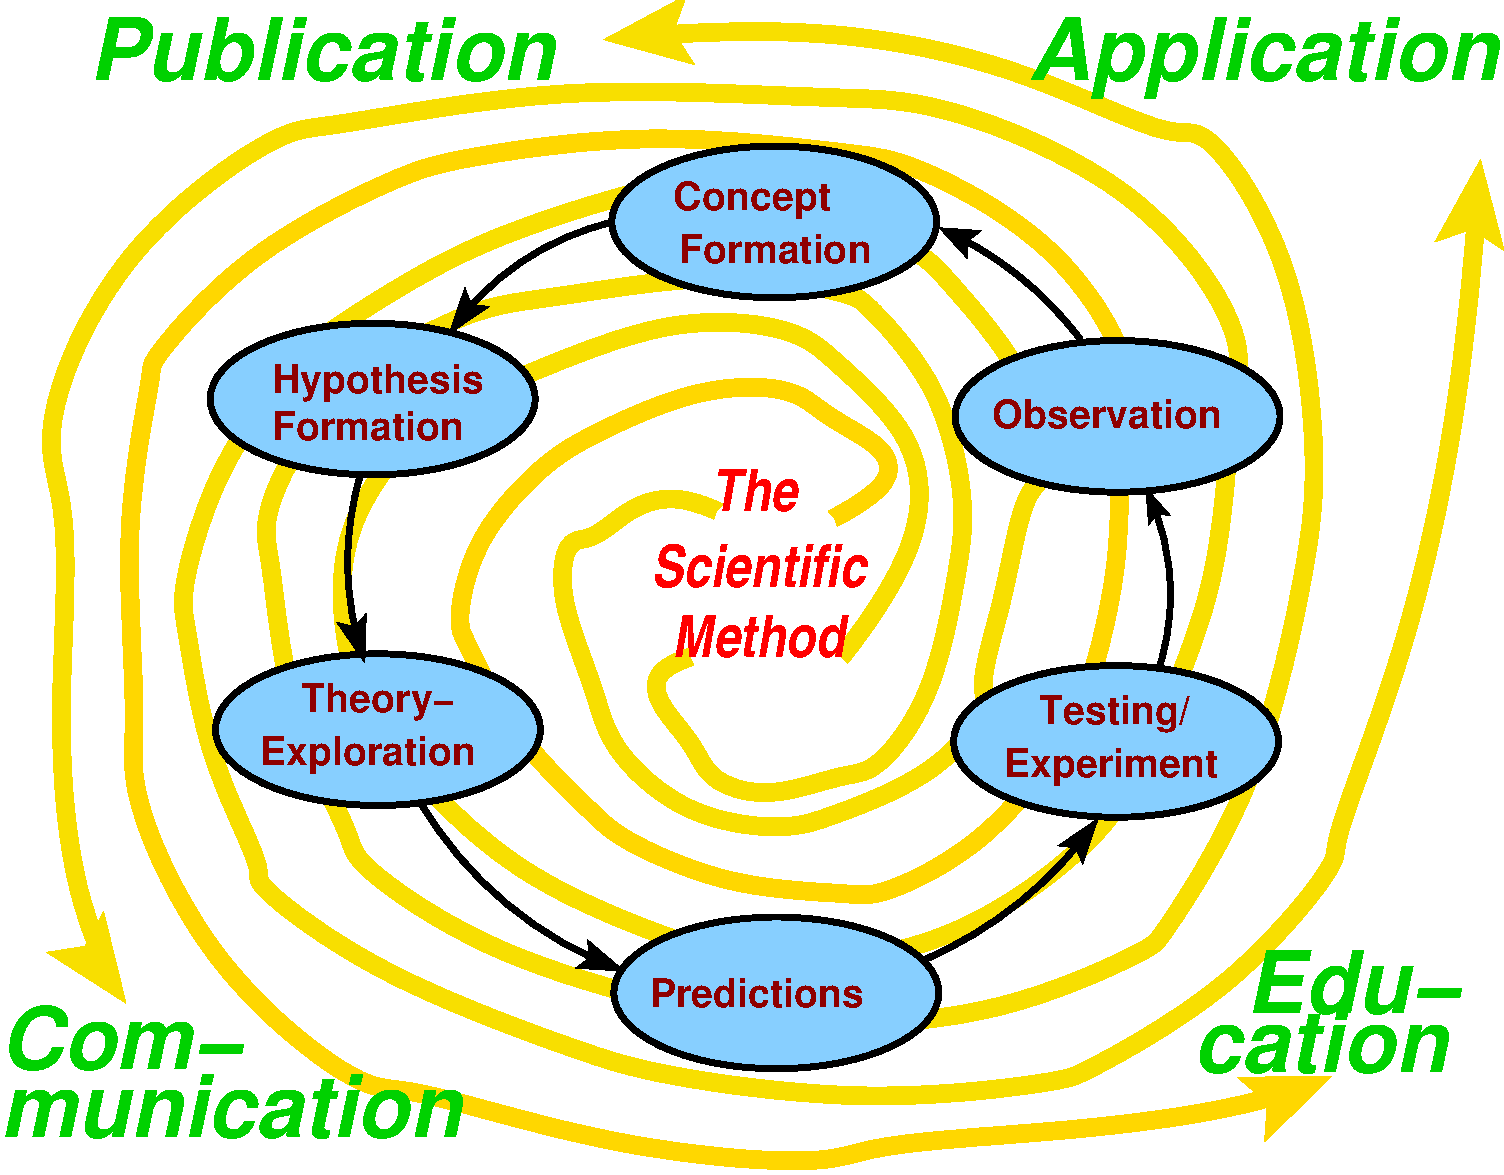
\includegraphics[width=6.5cm]{sci-method}\vspace{-.3cm}
  \caption{The Scientific Method}\label{fig:nw-Methode}\vspace{-.6cm}
\end{wrapfigure}
To further this vision we need to develop, implement, and provide semantic-based and
context-aware techniques for acquiring, organizing, processing, sharing and using
knowledge in science.
 
Our starting point is the view of the {\emph{scientific method}} as a spiral (see
Fig.~\ref{fig:nw-Methode}), where we have our focus on physics here.  In this view,
scientific research in physics moves in a spiral trajectory from original ideas to results
and even applications. Ideas pass through the processes of observation of natural
processes, then of concept formulation to describe these. These allow scientists to
express initial theories about (quantitative laws of nature governing) them, which are
then explored (what are the consequences of the model assumptions) leading to predictions
about processes that can be verified or falsified (to a certain degree) experimentally.
These experiments usually lead to new observations, starting the next round in the spiral
until a quantitative (mathematically formulated) \textit{theory} predicting exclusively
correct results from experiments is formulated.  Observables in physics have to be
suitably found such that they can be physically measured, their algebraic counterparts
being then candidates for building stones of a theory.  The semantics of mathematics as
such is more confined, searching for logically correct sets of rules.

At the moment, most of the steps in Fig.~\ref{fig:nw-Methode} are separately supported by
software systems, e.g.  literature searches in {\googlescholar} or {\wikipedia}, theory
exploration in computer algebra systems like {\mathematica}, and experiments in simulation
systems. But the systems are, by and large, not able to inter-operate since they use
differing data formats, make differing model assumptions, and are bound to an implicitly
given context that is only documented in publications about the systems. For instance,
copy-and-paste from {\googlescholar} or {\wikipedia} to {\mathematica} or a simulation
system is impossible because of this format problem. Moreover, where possible, copy and
paste can be very dangerous, since computer algebra systems make differing assumptions on
the Computer code-libraries, 
the simulation systems are based on\footnote{A simple example, where the lack of
explicit context led to a very expensive failure was the September 1999 loss of a \$125
million Mars orbiter, which crashed on Mars. The cause was that NASA used for its
specifications metric units, but the Lockheed Martin engineers misinterpreted the data
assuming they were given using Imperial units of measurement.}.

We are set here to arrive at a content markup format for science and technology by
extending the {\omdoc} ({\underline{O}pen} {\underline{M}athematical}
{\underline{Doc}uments}) format~\cite{Kohlhase:omdoc1.2} by an infrastructure for various
scientific domains. Since we can now share all the infrastructure --- in particular the
theory and statement levels --- with mathematics, the language design for {\physml}
becomes feasible.

\section{Something Enlightened Here}

The contributions of the network will emphasize language standardization and
context/domain modeling (as a semantic technique) and the added-value services that feed
on these representations. Note that language standards that encompass explicit
context/domain models are extensible and allow dynamic management of communication
contexts. The explicit context models represent the respective {\emph{domain knowledge}}
and support machine-supported knowledge management through its explicit structure.  We
distinguish three main paradigms which essentially differ in the depth of modeling the
domain knowledge, the coverage/scalability, and the formalisms employed.

First, the {\emph{Semantic Web}} is an approach that should be web-scalable in
principle.  However, the underlying context knowledge must be provided in an ontology
formalism like {\owl}~\cite{McGvHa:owl04}. This representation format is intentionally
limited in its semantic expressiveness, so that inference stays decidable and
web-scalable. Scientific knowledge can be only approximated very coarsely using this
approach so far.

Secondly, {\emph{Formal Methods}} use semantic formats with highly expressive
knowledge representation components. They can currently be used for high-security
applications only such as formal program verification, since they require the commitment
to a particular logical system, and the mathematical-logical formalization needed for
formal verification is extremely time-consuming.

Thirdly, specifically for mathematics there is the approach of structural/semantic markup
using formats such as {\openmath}~\cite{BusCapCar:2oms04},
{\mathml}~\cite{CarIon:MathML03}, and {\omdoc} ({\underline{O}}pen
{\underline{M}}athematical
{\underline{Doc}}uments~\cite{DBLP:conf/aisc/Kohlhase00,Kohlhase:omfmd05}). These
mathematical representation languages are now used in a large set of projects in automated
theorem proving, eLearning, ePublishing, and in formal digital libraries. They build on a
semantic representation format for mathematical formulae ({\openmath} objects or Content
{\mathml} representations) and extend this by an infrastructure for context and domain
models from ``formal methods''. In contrast to those, these structural/semantic approaches
do not require the full formalization of mathematical knowledge, but only the explicit
markup of important structural properties. For instance, a statement will already be
considered as ``true'' if there is a proof object that has certain structural properties,
not only if there is a formally verifiable proof for it. Since the structural properties
are logic-independent, a commitment to a particular logical system can be avoided without
losing the automatic knowledge management which is missing for semantically unannotated
documents. Of course such representations support only structural plausibility checks for
quality management (see section~\ref{sec:quality-management}) instead of full
verification. Work on the {\omdoc} format shows that most added-value services in
knowledge management do not need tedious formalization, but can be based on the
structural/semantic level. It is a major aspect of our work that we do not take the
all-or-nothing approach of the traditional theorem proving community that we either
guarantee full correctness of a theorem, or do not give any support. It is the main
objective of MKM to provide added value, which supports users on different levels of
precision.

We are assuming a three-layered structure model for semantic representation
formalisms:\label{page:levels}

\begin{description}
\item[Object level:] represents objects such as complex numbers, derivatives, etc for
  mathematics, map specifiers for geo-sciences or observables for physics.  Semantic
  re\-presentation formats typically use functional characterizations that represent
  objects in terms of their logical structure, rather than specifying their presentation.
  This avoids ambiguities which would otherwise arise from domain specific
  representations.
\item[Statement Level:] (natural/social/technological) sciences are concerned with
  modeling our environment, more precisely with statements about the objects in it. We can
  distinguish different types of statements: model assumptions, their consequences,
  hypotheses, and measurement results. All of them have in common that they state
  relationships between scientific objects and have to be verified or falsified in
  theories or experiments.  Moreover, all these statements have a conventionalized
  structure, such as Exercise, Definition, Theorem, Proof, and a standardized set of
  relations among each other. For instance, a model is fully determined by its assumptions
  (also called {\emph{axioms}}); all consequences are deductively derived from them (via
  {\emph{theorems}} and {\emph{proofs}}), and therefore their experimental falsification
  uncover false assumptions of the model.
\item[Theory/Context Level:] Representations always depend on the ontological context;
  even the meaning of a single symbol\footnote{e.g. the glyph $h$ as the height of a
    triangle or Planck's quantum of action.} is determined by its context, and depending
  on the current assumptions, a statement can be true or false. Therefore the sciences
  (with mathematics leading the way) have formed the habit to fix and describe the
  situation of a statement. Unfortunately, the structure of these situation descriptions
  remain totally implicit, and can therefore not be used for computer-supported
  management. Semantic representation formats make this structure explicit. For instance
  in mathematical logic, a theory is the deductive closure of a set of axioms, i.e. the
  (in general infinite) set of logical consequences of the model assumptions. Even though
  this fully explains the phenomenon context in theory, important aspects like the re-use
  of theories, knowledge inheritance, and the management of theory changes are disregarded
  completely. Therefore, formalisms with context level use elaborate inheritance
  structures for theories, e.g. in form of ontologies in the Semantic Web or in form of
  ``algebraic specifications'' in program verification.
\end{description}

An important trait of the three-layer language architecture is the inherent dependency
loop between the object- and theory levels mediated by the statement level: the objects
obtain their meaning from the theories their functional components are at home in, and the
theories are constituted by special statements, and in particular the objects that are
contained in them. This structure implicitly pervades the scientific discourse (hence the
name ``scientific method'') and the whole corpus of scientific knowledge. To make these
structures explicit enables the mechanization and automation of knowledge management
and the unambiguous, flexible communication of mathematical objects and knowledge that is
needed for meaningful interoperability of software systems in science. 


Many of the main results in mathematics have been triggered by ``{\emph{changes
    of representation}}'', e.g. calculus evolved out of the synthesis of geometry and
algebra. The ability to model context change and identify semantics at the same time is
essential for the adequate characterization of mathematical knowledge, we will discuss two
representative problems here:
  
(1) {\emph{Extension of notation-independent semantic encodings}.} Whether the parabola
function is represented as $t \rightarrow t^2$ or as $f(u)=u^2$ does not throw a human
reader off, she decodes the notation and transforms into her (private) nomenclature
$y=x^{2}$. However automated Internet searches, querying for a
second-order polynomial would be doomed here. 
  
(2) {\emph{Resolution of notational ambiguities}.} Conversely, mathematicians often use a
symbol ambiguously to encode {\emph{differing semantic contents}}. If we consider the
symbol ``$-$'', then this glyph can be interpreted as a (binary) {\emph{subtraction
    operator}} or as a (unary) {\emph{sign operator}}. In this case, the conflict can be
resolved in most cases, since the sign operator takes one argument whereas the subtraction
operator takes two. In mathematical practice, the inherent semantic structures are much
more complex, and as a consequence, semantic resolution presupposes deep understanding of 
mathematics and can only be partially automated. 

Such problems have been discussed in mathematics as part of the ``Grundlagen debate''
\cite{Giaquinto} (the debate about the logical/epistemological foundations of mathematics)
as early as the beginning of the last century, and have become technically relevant
e.g. for computer algebra systems (CAS). The results of these discussions have entered
document management paradigms as mandates for functional/semantic mark-ups. It is not for
nothing that paradigm-forming text formatting systems like {\xml} have been driven
significantly by the development of {\mathml} (the first {\xml}-based language in W3C).

We consider the syntax/semantics problems for mathematical knowledge to be solved in
principle by the development of computational logics\footnote{e.g. as funded by the EU in
  the CologNet network in the FET programme\cite{URL:colognet}).} and representation
formats like Content {\mathml}, {\openmath} or {\omdoc}. What remains is the problem of
{\emph{scaling the semantic representations}}, i.e. the tension between what is possible
in principle and what is necessary for the user.  In particular, neither pure nor applied
mathematics have been developed with respect to the inherent semantic phenomena. The
proposed network of excellence provides a forum for those European researchers that are
involved in making this happen for mathematics and those who want to transfer the
techniques from mathematics to general sciences.


\section{From Research to Practice}

Playing to the strengths of the network, MKM will be explicitly developed for three new
domains, namely, physics, geo-services and software engineering. Preliminary case studies
using {\openmath} and {\omdoc} suggest that the mechanisms for context/domain modeling are
largely sufficient for these domains. This is not surprising, since the view of the
scientific method is largely trans-disciplinary. On the object level, specialized
representation formalism for the respective study objects must be integrated.  The
consortium will accomplish this for selected application areas, chosen to be different
enough to show the generality of the approach:
\begin{itemize}
\item In physics, we need representations for measurable quantities
  (``observables''\cite{PML:web}\cite{Sev:physml}) and their induced algebraic and
  physical properties.  As an example, the {\emph{wording}} ``temperature'' in physics
  means the equilibrium thermal heat index.  Its {\emph{definition}} is the experimentally
  setup ``thermometer'' for measuring it.  It is a {\emph{continuous scalar coordinate}}
  in the thermostatic state-space.  It forms an affine space, with value zero excluded.
  Its dimension is {\emph{energy}} in the range of the thermometer scale.  Some physics
  laws (true statements) go with it: only finite energy systems can have negative values;
  there is only one such variable (first law of thermostatics); {\emph{entropy}} is
  related to it via the equation $\partial E / \partial S := T $.  The temperature is one
  of the variables of the thermostatic state-space where physics relations (laws) come in
  terms of partial derivatives of ``potential'' functions.
  
\item Geo-raster services are becoming increasingly important as multi-Terabyte archives
  are technically feasible but need more semantic knowledge to allow user-oriented
  queries.  This does not (yet) aim at image content understanding techniques (which are
  not suitable), but deriving raster map products like vegetation index, cross sections
  through atmospheric data cubes, and semantic aggregation. Ground truth data like
  satellite imagery have to be ornamented with information like their spatial coordinate
  systems, spatial and temporal extent of map layers, and their semantics (such as land
  use, satellite maps with some spectral bands, water areas - all of which have national
  and regional encoding rules).  The consortium will use {\omdoc} to augment geo-raster
  data context representation and assess the resulting added-value services in operational
  systems, such as the IRCCM (International Research Consortium on Continental Margins)
  database.
\item Documents in the scientific-technical domain, but also in other fields, regularly
  contain graphics-encoded information in the widest sense, such as tables, diagrams, and
  images (essentially, these also form "raster data", i.e., multi-dimensional arrays).
  Instead of providing links from the text corpus into some directory containing rendered
  raster images, the consortium's approach is to directly link the ground truth data (such
  as observations and measurements) and augment them using {\omdoc}. Based on this
  extended semantics, content-based search techniques will be developed and implemented
  which allow to search on the ground truth measurement data and return, e.g., matching
  documents.
\item In software engineering, formal methods are being increasingly used to provide
  guarantees of safety and reliability in critical software systems. Formal SE methods
  have at their core formal logical systems just like mathematics and like formal
  mathematics these systems are embodied in tools and methodologies. Inasmuch as MKM will
  be concerned about the management of formal mathematics, there should be natural, and
  possibly even rapid, transfer of MKM results to support for structuring mechanisms,
  abstraction and interoperability in formal methods in SE. As such, SE is an excellent
  domain in which to test the generic nature of MKM tools.
\item In Chemistry, the primary object in ChemML, the Chemical Markup Language
  concept~\cite{ISN:murray-rust}, is the {\emph{name}} of the molecule, with its physical
  and chemical properties, and reaction data attached. It is linked to graphical
  representations of the space distribution of atoms, their properties, etc
  \cite{Hilf:aud}.
\end{itemize}

It is plausible to assume that the extended representation facilities for natural sciences
and the enabled added value services will change the scientific method itself in
unforeseeable ways. In the literature we find slogans like ``redefining research'' or
``revisioning science'' for this. The extension of MKM for Knowledge Management for
E-Science has the potential to be a new {\emph{semantic}} basis for the communication
between scientists, between scientific software systems, and between man and machine. In
this, the {\emph{object level}} of knowledge (see below) provides the unambiguous
representation of scientific objects, and the {\emph{context level}} the representation of
the respective environment in which they are used.

Referring to the representation framework, the existing representations used will be
extended by an infrastructure for ``{\emph{Observables}}'' (from the abstract theory of
measurement\cite{ISN:qmech}\cite{ISN:einf}, ``{\emph{Raster Data}}'' (Results and data
from experiments or simulations, e.g.  in geo-services) and ``{\emph{Program Code}}'' (for
SE) to be able to cover knowledge from these disciplines. With these (and later possibly
additional) extensions to the languages we do not primarily aim for a full formalization
of the new object types, but for markup systems for the relevant structural properties
that allow to identify and reference the objects unambiguously, to make their context
dependence and their contribution to context explicit. Our scientific hypothesis in this
network is that with these extensions the infrastructure developed for mathematical
knowledge management at the theory and object level is already sufficient for representing
the broader sciences. The only exceptions might be ``descriptions of experiments'' that
ontologically probably belong to the statement level rather than on the object level. To
clarify this on the theoretical level is one of the goals of the interaction in the
network.

We see mathematical knowledge management techniques as an {\emph{enabling technology}},
that will put the cooperation between scientists, software systems, scientific
publication, navigation, and archiving of results onto a new (semantic) basis. We can
currently not envisage the full consequences of this technology, but we will explore the
breadth of the possible applications by a set of case studies from the disciplines
represented in the network. The network will study semantic, trans-disciplinary search
engines, methods for automated quality assertion for documents, and added-value services
based on knowledge. The materials developed in the network will be made accessible to the
scientific public by a semantic repository, to entice them to collaborate. We want to
develop a notion of {\emph{enlivened documents}} in which mathematical formulae are
directly coupled with computational rules, in which notations can be personalized, and
changes of representation can be automated, and in which for interpreted figures the
experimental raw data can be accessed transparently.


\section{Conclusion and Further Work}\label{sec:conclusion}

We have demonstrated that a Markup Language for the {\emph{content}} of physics can be
designed by extending the content and context markup format {\omdoc} with a
representational infrastructure for the principal objects of physics: observables,
systems, and experiments. The resulting language {\physml} is able to catch the logical
and operational structure specific to physics, differentiating this field from others. The
extension presented in this paper is part of the ongoing enterprise to extend the {\omdoc}
format to the {\bf{STEM}} fields ({\underline{S}}ciences, {\underline{T}}echnology,
{\underline{E}}ngineering and {\underline{M}}athematics).


The next step is now to evaluate the language by marking up a larger body of knowledge in
physics in {\physml}.  We have started work on the technically ubiquitous and basic field
of thermostatics. This should give us a clear indication whether {\physml} is adequate for
all of physics, or pinpoint the necessary changes to the language design.  An
international collaboration on the further development of {\physml} is looked for,
including experts from theoretical and applied physics and related fields, in particular
mathematics and chemistry.

New and powerful services can be implemented once the scientific content can be
semantically encoded, retrieved, and reused digitally.  In physics, these include the
search for other experiments on the same observables, dimension and algebraic checking of
mathematical equations, mapping to other mathematical representations of the same
theoretical physical expression, etc.

Using the approach of analyzing the operational and logical practices of a scientific
discipline field, and map this to field-specific modules extending the semantic markup
language {\omdoc} will allow to spread semantic content markup to other scientific fields.

With authors to increasingly make use of markup languages, and retrieval engines
following suit to offer intelligent search algorithms making use of the known markup
languages, users will gain effective tools to increase the reach-out of their scientific work,
having the {\emph{content}}, not just the text, of the work of others at their fingertips.


\bibliographystyle{alpha}
\bibliography{systems,crossrefs}
\end{document}

%%% Local Variables: 
%%% mode: latex
%%% TeX-master: t
%%% End: 



% LocalWords:  Eberhard Hilf Heinrich Stamerjohanns SVN fied stex GIS uments
% LocalWords:  athematical geo Grundlagen CAS CologNet FET multi IRCCM ChemML
% LocalWords:  revisioning ciences echnology ngineering athematics crossrefs
